% Requires TikZ; a schematic template, not measured data.
\begin{figure}[t]
\centering
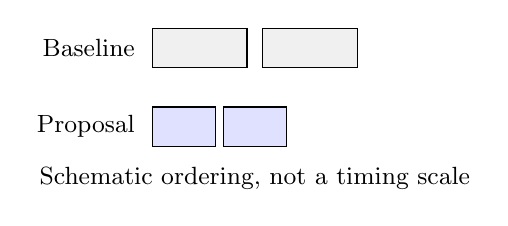
\begin{tikzpicture}[x=1cm,y=1cm,font=\small]
\draw[fill=gray!12] (0,1) rectangle (1.2,1.5);
\draw[fill=gray!12] (1.4,1) rectangle (2.6,1.5);
\node[anchor=east] at (-.1,1.25) {Baseline};
\draw[fill=blue!12] (0,0) rectangle (.8,.5);
\draw[fill=blue!12] (.9,0) rectangle (1.7,.5);
\node[anchor=east] at (-.1,.25) {Proposal};
\node at (1.3,-.4) {Schematic ordering, not a timing scale};
\end{tikzpicture}
\caption{\textbf{Comparison placeholder.} Replace schematic blocks with the actual baseline and changed schedule, ownership or data movement. Use measured widths only when timing data exist.}
\label{fig:contrast}
\end{figure}
